\section{Test Engine Fundamentals}

Microprocessors comprise diverse subsystems:
\emph{arithmetic-logic units} (\emph{ALU}), \emph{memory management units} (\emph{MMU}), \emph{branch processing units} (\emph{BPU}), etc.
Each subsystem requires specific \emph{test generation techniques} to cover the related functionality, including in particular \emph{corner cases}.
For example, it may be useful to produce an arithmetic overflow in the ALU, a page miss in the MMU, a mispredicted branch in the BPU, or the like.
To be able to discover ``high-quality'' bugs in the pipeline control logic, one needs to combine various techniques;
this allows creating complex test cases, which involve multiple microarchitectural events.

TPGs for different subsystems are often developed as independent tools;
thus, it is rather difficult, not to say impossible, to make them work together and to maintain the overall TPG environment.
In this work, we propose a solution having been implemented in MicroTESK (Microprocessor TEsting and Specification Kit),
a framework for constructing TPGs based on \emph{instruction set architecture} (\emph{ISA}) specifications.
The idea is as follows.
MicroTESK's core produces \emph{abstract test cases}, which are instruction sequences to be concretized (with particular test data, initialization code, etc.).
Each test case is decomposed into parts according to the opcodes and other information; the parts are scattered among the subsystem-specific \emph{engines}.
Each of them handles its part by applying the underlying techniques for test data generation.
Finally, the core composes the partial results into the \emph{concrete test case}.

\emph{Test engine} is a component that takes an abstract test case as an input and produces a series of \emph{concrete test cases},
i.e. instruction sequences with fully defined structure and behavior.
The concretization process consists of the following steps:

\begin{itemize}
\item
constructing constraints for test situations;
\item
solving the constraints and generating test data;
\item
creating the initialization code.
\end{itemize}

Constraints of the coverage model are stored in a database.
Given test situations, the engines access the storage to select the relevant constraints.
Basically, a situation is linked with a single constraint, e.g., $IntegerOverflow$.
In general, however, a situation maps to a family of constraints.
In this case, the engine either selects a random constraint from the family or tries each of them (or does something in between).

A test case's constraints are processed in the same order as the instructions are executed.
When a new instruction is about to run, the previous ones are executed in the ISS on a temporary context.
This execution phase, called \emph{presimulation}, allows taking into account dependencies between instructions.
The current constraint is strengthened with the context-related information (register values, memory data, etc.) and solved.
As a result, test data are generated and the initialization code is constructed.

\section{Test Engine Composition}

An important thing is that MicroTESK does not have a monolithic core;
instead, the test generation logic is decomposed into a number of engines, each being responsible for handling specific types of instructions and test situations.
The problem is how to integrate multiple engines solving different tasks into a single framework.
Our goal is to create a \emph{modular} TPG,
which means the ability to create self-contained extensions (plug-ins) that describe all modeling and testing aspects of the related subsystems and
the ability to register them in a black-box manner, without modifying the TPG's source code.

MicroTESK has a modular architecture that allows creating and registering TPG plug-ins.
Each of them consists of the following components:

\begin{itemize}
\item
the \emph{specification parser} (optional);
\item
the \emph{test engine}(\emph{s});
\item
the \emph{TDL extension}(\emph{s}) (optional).
\end{itemize}

A plug-in's parser analyzes specifications of the related subsystem and creates components that extend the microprocessor model.
For example, the \textsc{mmuSL} parser builds the MMU coverage model and the ISS extension for simulating address translation and caching.
These components are integrated into the model by using \emph{extension points}.
E.g., the ISS extension is registered as a \emph{memory access callback}.

\subsection{Test Engine Architecture}

Since test engines are capable of processing only particular instructions, test cases need to be split into parts and scattered among the engines.
An engine does not care whether it handles the entire test case or its part:
it looks through the instructions and generates constraints for the linked test situations;
when all engines have completed, MicroTESK starts processing the sequence by doing presimulation and applying engine-specific solvers and preparators.
Accordingly, each test engine consists of the following components:

\begin{itemize}
\item
the \emph{instruction selector};
\item
the \emph{constraint generator};
\item
the \emph{constraint solver};
\item
the \emph{initialization code constructor}.
\end{itemize}

Provided that there are two engines, $A$ and $B$ (except for the default one), let us consider the overall scenario in more detail (see Fig.~\ref{multiple-engines}).
Given an abstract test case $T = \{\langle I_i, S_i \rangle\}_{i=1}^n$,
where for each $i$, $I_i$ is an instruction and $S_i$ is a test situation,
the engines select subsequences:

\vspace{2mm}
$T_E \equiv \{\langle I_{i_j}, S_{i_j} \rangle\}_{j=1}^{n_E} \leftarrow Select_E(T)$, where $E \in \{A, B\}$.
\vspace{2mm}

$T_A$ and $T_B$ may overlap and are allowed not to cover $T$ (uncovered items are processed by the default engine).
Each engine looks through the sequence and generate the corresponding constraints.
In addition, an engine may add prologues and epilogues to the instructions being processed
(if there are loops, it may be useful to do some data modifications):

\vspace{2mm}
$\textbf{T}'_E \equiv \big{\{}\{\langle (\alpha_{i_j}^k, I_{i_j}, \omega_{i_j}^k), C_{i_j}^k \rangle\}_{j=1}^{n_E}\big{\}}_{k=1}^{N_E} \leftarrow Process_E(T_E)$.
\vspace{2mm}

Here, for each $k$ and $j$, $\alpha_{i_j}^k$ is a prologue, $\omega_{i_j}^k$ is an epilogue, and $C_{i_j}^k$ is a constraint.
Typically, $\alpha_{i_j}^k=\omega_{i_j}^k=\varepsilon$ (no prologues and epilogues are provided) and $N_E=1$.

The \emph{combinator} component is used to select some sequences (in particular, all) from the Cartesian product $\textbf{T}'_A \times \textbf{T}'_B$:
$$\textbf{T}' \leftarrow Combine(\textbf{T}'_A, \textbf{T}'_B).$$

For each combination $(T'_A, T'_B) \in \textbf{T}'$, its sequences, i.e. parts processed by the engines, are \emph{merged} into a single one:
$$T' \equiv \{\langle I_i, C_i \rangle\}_{i=1}^m \leftarrow Flatten(Join(T'_A, T'_B)).$$
Merging is done in two steps:

\begin{itemize}
\item
joining the sequences with prologues and epiloges inside;
\item
flattening the resulting sequence.
\end{itemize}

The first step is straightforward unless the sequences overlap.
If items $\langle (\alpha, I, \omega), C \rangle$ and $\langle (\alpha', I, \omega'), C' \rangle$ are to be put into the same position, the result is as follows:
$$\langle (\alpha \cdot \alpha', I, \omega \cdot \omega'), C \wedge C' \rangle,$$
where $\cdot$ is catenation, and $\wedge$ is conjunction.

The purpose of the second step is to deattach prologues and epilogues from the instructions and append them into the sequence.
Each item $\langle (\{I_{\alpha_i}\}_{i=1}^s, I, \{I_{\omega_i}\}_{i=1}^t), C \rangle$ is ``unrolled'' to the following sequence:
$$\{\langle I_{\alpha_i}, \epsilon \rangle\}_{i=1}^s \cdot \{\langle I, C \rangle\} \cdot \{\langle I_{\omega_i}, \epsilon \rangle\}_{i=1}^t,$$
where $\epsilon$ denotes the null constraint.

The sequence $T'$ is still abstract and needs to be concretized.
The concretization process is as usual; the only peculiarity is that engine-specific components are used to solve constraints and generate initialization code.
$$T'' \leftarrow Init\big{(}Solve(C_1)\big{)} \cdot ... \cdot Init\big{(}Solve(C_m)\big{)} \cdot \{I_i\}_{i=1}^m.$$
Note that $Init\big{(}Solve(\epsilon)\big{)}=\varepsilon$ (no test data and initialization code is produced for null constraints).
The result is a concrete test case to be written into a file.

\begin{figure}
\centering
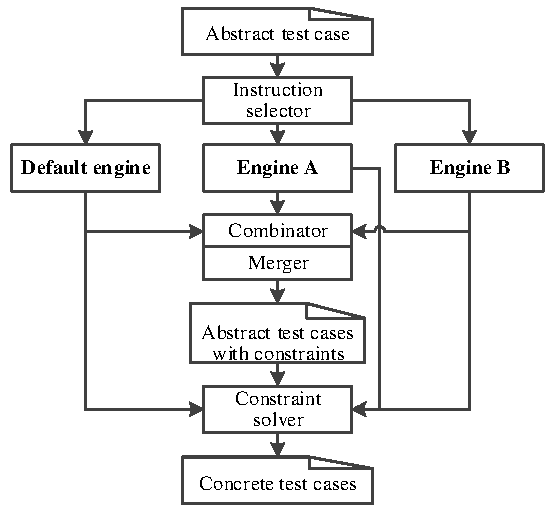
\includegraphics [width=0.9\textwidth]
{engines.pdf}
\caption{Test case processing with multiple engines}
\label{multiple-engines}
\end{figure}

\subsection{Template Description Language Extension}

Test engines and test situations have attributes used to set up their processing modes.
To pass those attributes to the TPG, a TDL extension is not usually required:
components can be easily configured by specifying the corresponding key-value pairs.
Here is an example, where the $engine$ attribute is used.

\begin{lstlisting}[language=ruby, emph={do, situation, end, engine, memory}]
sw r1, 0x0, r2 do # sw r1, 0x0(r2) (store word)
  # This situation is processed by the memory engine
  situation('memory', :engine => :memory)
end
\end{lstlisting}
It may be useful to introduce ``syntactic sugar'' methods,
which construct objects to be used as attribute values.

\begin{lstlisting}[language=ruby, emph={do, situation, end, path, constraints, hit, miss, eq, event}]
sw r1, 0x0, r1 do
  situation(
    ...
    :path => constraints(
      hit('JTLB'),       # Hit in JTLB (Joint TLB)
      eq('JTLB.V0', 1),  # Validity bit is set
      event('L1',        # L1 hit/miss event is randomized
        :hit  => 70,     # 70% probability of L1 hit
        :miss => 30))    # 30% probability of L2 miss
      )
end
\end{lstlisting}

To construct initialization code, test engines use preparators.
Most of them, such as register and memory preparators, are engine independent.
However, some engines need more.
For example, the $memory$ engine uses preparators for initializing translation lookaside buffers (TLBs), page tables, etc.
To support new types of preparators, one should implement and register a TDL extension.
Such extensions consist of the following parts:

\begin{itemize}
\item
the \emph{Ruby module} introduces language facilities for describing preparator templates;
\item
the \emph{TPG module} produces initialization code by instantiating the preparator template for given test data.
\end{itemize}

MicroTESK's core implements the $default$ engine that solves constraints extracted from nML specifications and constructs initialization code by using register and memory preparators.
Currently, there are two extensions: $branch$ and $memory$.
The first one is responsible for handing branch instructions and creating various execution traces.
The second one is aimed at processing memory accesses.

The test template below demonstrates how multiple engines ($default$, $branch$, and $memory$) can be used together.
There is a control flow structure formed by BPU instructions and filled with MMU and ALU instructions.
The $branch$ engine handles the BPU instructions and creates constraints on execution traces.
The $memory$ engine handles the MMU instructions and creates constraints describing memory access scenarios.
The $default$ engine handles the ALU instructions and picks up constraints given in the linked test situations.
The number of constraint combinations produced by the $branch$ and $memory$ engines is limited in their settings.
Test cases produced by different engines are combined together with the help of the $product$ combinator,
generates the Cartesian product, i.e. all possible combinations, of the given sets of partial test cases.

\begin{lstlisting}[language=ruby, emph={sequence,
                                        situation,
                                        engines,
                                        combinator,
                                        branch,
                                        branch_exec_limit,
                                        trace_count_limit,
                                        memory,
                                        classifier,
                                        page_mask,
                                        align,
                                        count,
                                        engine,
                                        stream,
                                        base,
                                        start,
                                        finish,
                                        normal,
                                        overflow,
                                        run
                                        }]
sequence (:engines => { # Engine combination
           :combinator => 'product',
           :branch => { # Branch engine settings
             :branch_exec_limit => 3,
             :trace_count_limit => 10
           },
           :memory => { # Memory engine settings
             :count => 5,
             :page_mask => 0x0fff
           }
         }) {
  label :start
    bgez s0, :normal do # BPU: branch if >= 0
      situation('bgez-if-then', :engine => :branch, ...)
    end
    nop                 # ALU: no operation
  label :overflow
    add t0, t1, t2 do   # ALU: add registers
      situation('IntegerOverflow')
    end
    j :finish do        # BPU: jump
      situation('b-goto', :engine => :branch)
    end
    nop                 # ALU: no operation
  label :normal
    add t0, t3, t4 do   # ALU: add registers
      situation('normal')
    end
    ld a0, 0x0, s4 do   # MMU: load double word
      situation('memory', :engine => :memory, ...)
    end
    sd a1, 0x0, s5 do   # MMU: store double word
      situation('memory', :engine => :memory, ...)
    end
  label :finish
    bltz s1, :start do  # BPU: branch if <= 0
      situation('bltz-if-then', :engine => :branch, ...)
    end
    nop                 # ALU: no operation
}.run
\end{lstlisting}
\vspace*{-0.1in}

